\section{Detector resolution}
\mbox{}\vspace{-\baselineskip}


Let's now assume that for all events in the sample the momenta of registered particles are determined within the uncertainty due to the detector resolution. Then the missing quantities $M_{X[0]}^{2}$ and $M_{X[\pi^{-}]}^{2}$ acquire some uncertainty as well, which is estimated below.


A missing quantity $M_{X}^{2}$ can be written in the following way,
\begin{equation}
\begin{aligned}
&M_{X}^{2}&=&~(E_{X})^{2} - (p_{X}^{x})^{2} - (p_{X}^{y})^{2}  -  (p_{X}^{z})^{2} \\
&&=&~\left (\sum_{\substack{i}} \pm \sqrt{m_{i}^{2}+p_{i}^{2}} \right )^{2} - \left (\sum_{\substack{i}}\pm p_{i}^{x} \right )^{2} - \left (\sum_{\substack{i}}\pm p_{i}^{y} \right )^{2} - \left (\sum_{\substack{i}}\pm p_{i}^{z} \right )^{2},\\
\end{aligned}\label{eq:mm_def2}
\end{equation}
where $E_{X}$ and $p_{X}^{j}$ ($j = x,~y,~z$) are the energy and momentum components of the missing four-vector, while $m_{i}$, $E_{i}$, and $p_{i}^{j}$ are the mass, energy, and momentum components of the individual particles with the index $i$ running over all particles involved in the missing mass calculation (see Eqs.~\eqref{eq:mm_def}). For the $\pm$ sign, the plus is taken for the initial particles ($e$ and $p$) and the minus for the final particles.



First, one can estimate the uncertainties of the quantities $E_{X}$ and $p_{X}^{j}$ through the momentum uncertainties of the individual particles. 
The absolute uncertainties for the energy components $E_{X}$ can be expressed by
\begin{equation}
\begin{aligned}
&\Delta E_{X[0]} &=&~\sqrt{ \left ( \Delta E_{e'} \right )^{2} + \left ( \Delta E_{p'} \right )^{2} +  \left ( \Delta E_{\pi^{+}} \right )^{2} + \left ( \Delta E_{\pi^{-}} \right )^{2}} \\
&&=&~\sqrt{\left ( \Delta p_{e'} \right )^{2} + \left (p_{p'}/E_{p'}\right )^{2} \left (\Delta p_{p'} \right )^{2} +  \left (p_{\pi^{+}}/E_{\pi^{+}}\right )^{2} \left (\Delta p_{\pi^{+}} \right )^{2}+\left (p_{\pi^{-}}/E_{\pi^{-}}\right )^{2} \left (\Delta p_{\pi^{-}} \right )^{2}}, \\[10pt]
&\Delta E_{X[\pi^{-}]} &=&~\sqrt{ \left ( \Delta E_{e'} \right )^{2} + \left ( \Delta E_{p'} \right )^{2} + \left ( \Delta E_{\pi^{+}} \right )^{2}}\\
&&=&~\sqrt{\left ( \Delta p_{e'} \right )^{2} + \left (p_{p'}/E_{p'}\right )^{2} \left (\Delta p_{p'} \right )^{2} +  \left (p_{\pi^{+}}/E_{\pi^{+}}\right )^{2} \left (\Delta p_{\pi^{+}} \right )^{2}},\\
\end{aligned}\label{eq:res}
\end{equation}
where $\Delta p_{i}$ is the uncertainty of the momentum magnitude for the particle $i$, which comes from the track momentum resolution of the Drift Chambers.

The absolute uncertainties for the momentum components $p_{X}^{j}$ are in turn given by
\begin{equation}
\begin{aligned}
&\Delta p_{X[0]}^{j} &=&~\sqrt{ \left ( \Delta p_{e'}^{j} \right )^{2} + \left ( \Delta p_{p'}^{j} \right )^{2} +  \left ( \Delta p_{\pi^{+}}^{j} \right )^{2} + \left ( \Delta p_{\pi^{-}}^{j} \right )^{2}}, \\
&\Delta p_{X[\pi^{-}]}^{j} &=&~\sqrt{ \left ( \Delta p_{e'}^{j} \right )^{2} + \left ( \Delta p_{p'}^{j} \right )^{2} +  \left ( \Delta p_{\pi^{+}}^{j} \right )^{2}},\\
\end{aligned}\label{eq:res2}
\end{equation}
where $\Delta p_{i}^{j}$ are the uncertainties of the components of the particle's momenta ($j~=~x,~y,~z$), which come from the track momentum and angular resolutions of the Drift~Chambers.


As follows from Eqs.~\eqref{eq:res} and~\eqref{eq:res2}, the absolute uncertainties of $E_{X[0]}$ and $p_{X[0]}^{j}$ are larger than those of $E_{X[\pi^{-}]}$ and $p_{X[\pi^{-}]}^{j}$, respectively, as the former quantities include extra terms associated with the additional registered particle (which is the $\pi^{-}$ here).


Now, using Eq.~\eqref{eq:mm_def2}, the absolute uncertainties of the missing quantities $M_{X[0]}^{2}$ and $M_{X[\pi^{-}]}^{2}$ can be estimated as the following,
\begin{equation}
\begin{aligned}
&\Delta M_{X[0]}^{2} &=&~\sqrt{ \left (2E_{X[0]} \Delta E_{X[0]} \right )^{2} + \sum_{\substack{j = x,~y,~z}}\left (2p_{X[0]}^{j} \Delta p_{X[0]}^{j} \right )^{2}}, \\
&\Delta M_{X[\pi^{-}]}^{2} &=&~\sqrt{ \left (2E_{X[\pi^{-}]} \Delta E_{X[\pi^{-}]} \right )^{2} +  \sum_{\substack{j = x,~y,~z}}\left (2p_{X[\pi^{-}]}^{j} \Delta p_{X[\pi^{-}]}^{j} \right )^{2}}. \\
\end{aligned}\label{eq:res3}
\end{equation}

In Eqs.~\eqref{eq:res3} the uncertainties $\Delta E_{X[0]}$, $\Delta p_{X[0]}^{j}$ and $ \Delta E_{X[\pi^{-}]}$, $\Delta p_{X[\pi^{-}]}^{j}$ are respectively comparable, though the former are systematically larger than the latter (as was shown above). Meanwhile, both $E_{X[0]}$ and $p_{X[0]}^{j}$ are very close to zero, while both $E_{X[\pi^{-}]}$ and $p^{j}_{X[\pi^{-}]}$ are non-zero. As a consequence, the quantity $M_{X[0]}^{2}$ acquires smaller absolute uncertainty value than $M_{X[\pi^{-}]}^{2} $. This is, however, not the case for their relative uncertainties because (in contrast to $M_{X[\pi^{-}]}^{2}$) the quantity $M_{X[0]}^{2}$ is extremely close to zero.


\begin{figure}[htp]
\begin{center}
\framebox{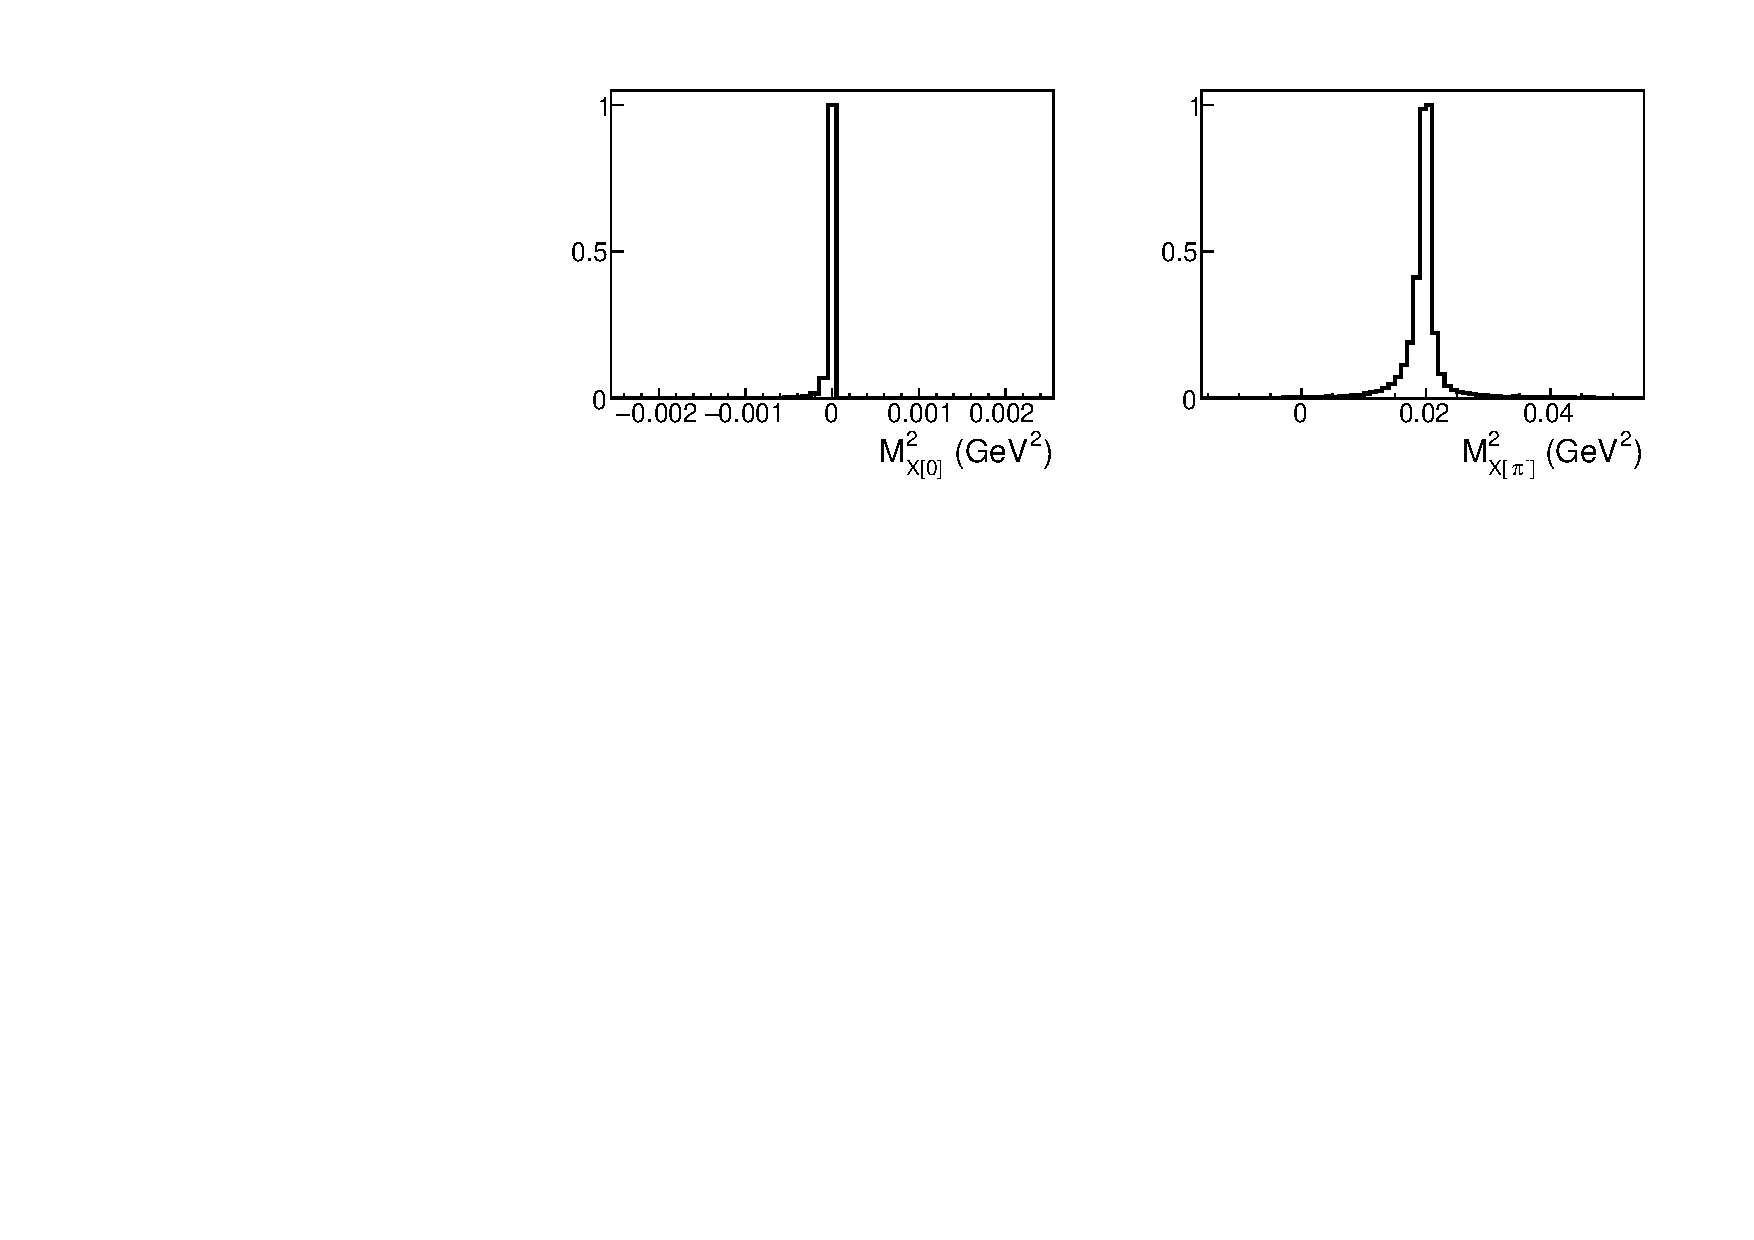
\includegraphics[width=\textwidth]{pictures/mm_res.pdf}}
\caption{\small Impact of the detector resolution on $M_{X[0]}^{2}$ (left) and $M_{X[\pi^{-}]}^{2}$ (right). The distribution of $M_{X[0]}^{2}$ is zoomed in on $x$ to demonstrate the disturbances. To produce these histograms, events generated with TWOPEG~\cite{twopeg} were reconstructed via the CLAS reconstruction software~\cite{Mecking:2003zu}.} \label{fig:mm_res}
\end{center}
\end{figure}

To simulate the impact of the detector resolution on the missing quantities, events generated with TWOPEG~\cite{twopeg} were reconstructed via the CLAS reconstruction software~\cite{Mecking:2003zu}. Figure~\ref{fig:mm_res} presents the resulting distributions, which illustrate the above calculations. As seen in the plots, the $M_{X[0]}^{2}$ distribution (left) turns out to be visually very narrow with slight disturbances, while the $M_{X[\pi^{-}]}^{2}$ distributions (right) acquires perceptible smearing\footnote[4]{Note that the detector resolution depends on particle kinematics~\cite{Mecking:2003zu}.}. 


